%% Springer Nature journal format — sn-mathphys-num (numbered references)
\documentclass[pdflatex,sn-mathphys-num]{sn-jnl}

%% ---- Standard packages ----
\usepackage{graphicx}
\usepackage{multirow}
\usepackage{amsmath,amssymb,amsfonts}
\usepackage{amsthm}
\usepackage[title]{appendix}
\usepackage{xcolor}
\usepackage{textcomp}
\usepackage{booktabs}
\usepackage{url}
\usepackage{enumitem}
\setlist[itemize]{label=\textbullet,leftmargin=1.5em,itemsep=2pt,topsep=3pt}
\hyphenation{Conformalized}
\usepackage{hyperref}
\hypersetup{colorlinks=true,linkcolor=blue,citecolor=blue,urlcolor=blue}

%% ---- Theorem styles ----
\theoremstyle{thmstyleone}
\newtheorem{theorem}{Theorem}
\newtheorem{proposition}[theorem]{Proposition}
\theoremstyle{thmstyletwo}
\newtheorem{example}{Example}
\newtheorem{remark}{Remark}
\theoremstyle{thmstylethree}
\newtheorem{definition}{Definition}

\raggedbottom

%% Fix ORCID logo macro (PDF version)
\renewcommand{\orcidlogo}{
\includegraphics[width=8pt]{Orcidlogo.pdf}}
\renewcommand{\orcid}[1]{\unskip\,\href{https://orcid.org/#1}{\orcidlogo}}

%% ============================================================
\begin{document}
%% ============================================================

\title[CLV Prediction Framework]{A Semantic Knowledge-Driven and Explainable Framework
for Customer Lifetime Value Prediction and VIP Targeting
in Online Retail}

%% ---- Author block ----
\author*[1]{\fnm{Vu Minh Anh} \sur{Nguyen}}\email{anhnvmse203412@fpt.edu.vn}

\affil*[1]{%
  \orgdiv{Department of Information Technology},
  \orgname{FPT University},
  \orgaddress{%
    \city{Ho Chi Minh City},
    \country{Vietnam}
  }
}

%% ---- Abstract ----
\abstract{Customer Lifetime Value (CLV) prediction in online retail
faces two simultaneous pathologies: zero inflation (47--67\% of
customers have zero future spend) and heavy-tailed non-zero
spending (skewness $>22$). We propose a \emph{semantic
knowledge-driven} and explainable framework that extends classical
temporal CLV modelling in three directions. First, we introduce
\textbf{semantic product graph features}: a co-purchase graph
encoded by Positive PMI and Truncated SVD yields customer taste
profiles that are statistically orthogonal to RFM
(Adjusted Rand Index $0.03$) and partition customers into six
interpretable taste-based segments ($p{=}4.5\!\times\!10^{-5}$);
these features enrich \textbf{interpretable taste segmentation}
(24.5\% of Stage-2 SHAP importance) and complement---rather than
replace---RFM-based CLV ranking signals.
Second, we compare 17 models on Online Retail~II (805{,}549
transactions, 5{,}038 customers, 24~months) under walk-forward
evaluation (three primary windows for the 17-model benchmark, all
five windows for the semantic and CQR analyses), showing that a
two-stage Hurdle Model achieves Normalized Gini $0.834$ (95\%
bootstrap CI [0.767, 0.883]) and 60.96\% Revenue Capture at top
10\%---comparable to recent deep CLV baselines---while remaining
fully interpretable. Third, we apply \mbox{Conformalized Quantile Regression}
(CQR) to the Hurdle Model, achieving 95.2\% empirical coverage at the
nominal 95\% level. Uncorrected MC-Dropout intervals from MCD-ZILN cover only
34.2\% of test values; split-conformal widening restores MCD coverage
to 94.7\%, confirming that heavy-tailed CLV requires explicit
calibration rather than nominal Bayesian intervals alone.
SHAP analysis identifies Monetary, M/T ratio and recent spending as
dominant predictors, with semantic dimensions accounting for 24.5\%
of Stage-2 importance.}

\keywords{Customer lifetime value, VIP targeting, Hurdle model, Explainable AI,
Semantic intelligence, Product graph embeddings, Conformalized quantile regression,
Walk-forward cross-validation, Zero-inflated distribution, Online retail analytics}

\maketitle

%% ============================================================
\section{Introduction}\label{sec:intro}
%% ============================================================

Customer Lifetime Value (CLV) prediction directly informs marketing
budget allocation, retention strategy, and personalised
engagement~\cite{fader2005rfm,gupta2006clv}: accurately identifying
high-value customers lets retailers focus scarce resources on the
segments most likely to generate future revenue. Throughout this paper, RFM acts as the descriptive segmentation
lens, predicted CLV as the ranking target, and walk-forward
Revenue Capture@$K\%$ as retention-style validation that top-ranked
customers actually return revenue in held-out windows.
The task is challenging because CLV is simultaneously
\emph{zero-inflated} (47--67\% of customers have zero future spend
in our windows) and \emph{heavy-tailed} (skewness $>22$), violating
MSE-regression assumptions and demanding specialised
approaches~\cite{wang2019deep}.

Classical CLV models (BG/NBD\,+\,Gamma-Gamma)~\cite{fader2005counting,
fader2013gammagamma} rely on summary RFM features; deep approaches such
as ZILN~\cite{wang2019deep}, OptDist~\cite{tang2024optdist},
dRNN~\cite{meta2024drnn}, and MCD-ZILN~\cite{mcd2024clv} vary in
interpretability and calibration. Three gaps persist: (i)~few comparisons
use leakage-free temporal evaluation; (ii)~the marginal value of sequence
and semantic features over tuned tabular methods is unclear; (iii)~nominal
95\% uncertainty intervals from MC Dropout cover only $\sim$34.2\% of
test CLV on our benchmark. This paper closes those gaps with six
contributions:

\begin{enumerate}
\item A \textbf{time-aware evaluation framework}: walk-forward CV
across five windows (9--21~months observation), bootstrap 95\% CIs
and paired $t$-tests.
\item A \textbf{semantic product graph} representation: a co-purchase
graph encoded by Positive PMI and Truncated SVD yields 32-dim
product embeddings; per-customer revenue-weighted profiles capture
latent product-taste knowledge orthogonal to aggregate RFM, with
$K$-means clusters that are statistically distinct in CLV
($p{=}4.5\!\times\!10^{-5}$) and only weakly aligned with RFM clusters
(ARI $0.03$).
\item A \textbf{comprehensive comparison of 17 models} on Online
Retail~II spanning seven families (baselines, probabilistic, linear,
gradient boosting, Hurdle, ZILN-family, sequence DL).
\item An \textbf{ablation study} of feature groups plus \textbf{two-stage
SHAP explainability} for both Hurdle stages.
\item \textbf{Supervised dimension selection} and \textbf{recency-aware
semantic profiling} that contribute 24.5\% of Stage-2 SHAP importance
and yield interpretable taste clusters orthogonal to RFM (ARI $0.03$),
without statistically significant aggregate NG gains ($p\geq 0.35$).
\item \textbf{Conformalized Quantile Regression
(CQR)}~\cite{romano2019conformalized} on the Hurdle Model, achieving
95.2\% empirical coverage; split-conformal calibration of MCD-ZILN
raises its coverage from 34.2\% to 94.7\%, isolating calibration---not
architecture---as the key uncertainty bottleneck.
\end{enumerate}

This work advances \emph{semantic intelligence} in retail analytics
by constructing product co-purchase graph embeddings that capture
latent customer taste profiles orthogonal to traditional RFM features.
The remainder of the paper covers related work
(Sec.~\ref{sec:related}), methodology (Sec.~\ref{sec:methodology}),
experimental setup (Sec.~\ref{sec:experiments}), results
(Sec.~\ref{sec:results}), and discussion plus conclusion
(Sec.~\ref{sec:discussion}--\ref{sec:conclusion}).

%% ============================================================
\section{Related Work}\label{sec:related}
%% ============================================================

\textit{Classical CLV models.} BG/NBD~\cite{fader2005counting} and
Gamma-Gamma~\cite{fader2013gammagamma} anchor non-contractual CLV
modelling but assume permanent churn and frequency--value independence.

\textit{Machine learning and deep CLV.} Tree ensembles with Optuna
tuning~\cite{akiba2019optuna} remain strong on tabular
data~\cite{grinsztajn2022treesvsnn}. Deep CLV methods include ZILN
loss~\cite{wang2019deep}, OptDist~\cite{tang2024optdist},
dRNN~\cite{meta2024drnn}, and MCD-ZILN~\cite{mcd2024clv}. Few prior
studies jointly address temporal leakage, fair deep-vs-tree
comparison, semantic product knowledge, and calibrated uncertainty.

\textit{Semantic intelligence.} Product co-purchase graphs form a
knowledge layer over transactions~\cite{bullinaria2007extracting,
levy2014neural,linden2003amazon}. We treat PPMI--SVD embeddings as
semantic profiles orthogonal to RFM, evaluated under walk-forward
protocol with two-stage SHAP.

\textit{Hurdle models and explainability.}
Hurdle architectures~\cite{mullahy1986specification,cragg1971statistical}
decouple purchase incidence from conditional spend. SHAP~\cite{lundberg2017unified}
and Normalized Gini~\cite{wang2019deep} support interpretability and
ranking evaluation respectively.

%% ============================================================
\section{Methodology}\label{sec:methodology}
%% ============================================================

The proposed framework comprises data cleaning, feature engineering,
walk-forward CV, model training, evaluation, VIP simulation, and
two-stage SHAP analysis.

\subsection{Problem Formulation}

Let $\mathcal{D} = \{(\mathbf{x}_i, y_i)\}_{i=1}^{N}$ denote the dataset,
where $\mathbf{x}_i \in \mathbb{R}^d$ is a feature vector summarising
customer $i$'s observation-window history, and $y_i \in \mathbb{R}_{\geq 0}$
is the actual revenue generated by customer $i$ during a future prediction
window. The CLV prediction task is to learn $\hat{f}: \mathbb{R}^d \to
\mathbb{R}_{\geq 0}$ minimising a chosen loss while preserving customer
ranking quality.

A central challenge is that $y_i = 0$ for a large fraction of customers
(non-returning buyers), while the non-zero values are heavy-tailed. We thus
formulate CLV as a mixture distribution:
\begin{equation}
P(Y = y) =
\begin{cases}
1 - \pi, & y = 0, \\[3pt]
\pi\, f_Y(y;\,\theta), & y > 0,
\end{cases}
\label{eq:mixture}
\end{equation}
where $\pi = P(Y > 0)$ is the purchase probability and $f_Y(y;\,\theta)$ is
the conditional density of positive values. Both the Hurdle Model and the
ZILN-family methods are instances of Eq.~\eqref{eq:mixture} that differ in
their parameterisation and training procedure.

\subsection{Temporal Walk-Forward Cross-Validation}

We use five non-overlapping walk-forward windows W1--W5, all
anchored at 2009-12-01, with observation/prediction horizons (in
months): \mbox{W1\,=\,12/3}, \mbox{W2\,=\,15/3},
\mbox{W3\,=\,18/6} (the primary 6-month-horizon window),
\mbox{W4\,=\,9/3} (shortest history), and \mbox{W5\,=\,21/3}
(longest history). Window sizes range from 3{,}313 to 5{,}245
customers and zero-rates from 42\% to 67\%. Within each window we
apply a stratified 80/20 train/test split preserving the VIP class
balance (top 10\% by actual CLV).

\subsection{Feature Engineering}

We construct 23 base features in four groups: \textbf{RFM} (Recency,
Frequency, Monetary; 3); \textbf{Behavioural} (Tenure, ActiveMonths,
ProductDiversity, AvgOrderValue, AvgDaysBetweenOrders, Regularity,
IsUK; 7); \textbf{Interaction} (log-Monetary, log-Frequency,
log-AOV, M/F, M/T, ActiveMonths/Tenure; 6); and \textbf{Monthly
sequence summaries} (mean, std, max, recent-3 mean and max,
active-month count, trend; 7). A fifth group, \textbf{Semantic
product-graph features} (Sec.~\ref{sec:semantic}), adds 8 supervised
top-correlation dimensions from the full profile plus 8 from a
90-day recency-aware profile, a drift scalar, and product counts.

\subsection{Proposed Two-Stage Hurdle Model}

\textit{Why a Hurdle architecture rather than a single XGBoost?}
A single MSE-trained regressor must optimise two conflicting
objectives---pulling predictions toward zero for the 47--67\%
no-purchase mass while tracking long-tail VIPs---under one loss.
The Hurdle decouples them, training one classifier on
\emph{whether} a customer returns and one regressor on
\emph{how much} a returner spends, each with the loss appropriate
to its sub-task. The single-loss baselines in Sec.~\ref{sec:results}
therefore act as ablations of components the Hurdle subsumes.

We decompose Eq.~\eqref{eq:mixture} into two LightGBM~\cite{ke2017lightgbm}
stages: a binary \textbf{classifier} estimating
$\hat{\pi}_i = P(y_i{>}0\mid\mathbf{x}_i)$ on all $N$ customers, and a
\textbf{regressor} estimating
$\hat{m}_i = \mathbb{E}[\log(1{+}y_i)\mid y_i{>}0,\mathbf{x}_i]$ on the
positive subset. The final prediction combines both with a lognormal
bias correction:
\begin{equation}
\hat{y}_i = \hat{\pi}_i \left(e^{\hat{m}_i} - 1\right)
             \exp\!\left(\tfrac{\hat{\sigma}^2}{2}\right),
\label{eq:hurdle}
\end{equation}
with $\hat\sigma^2$ the validation residual variance of the log-target on
positive customers (a homogeneous lognormal correction; heteroscedastic
Stage-2 modelling is left to future work); both stages use early stopping.

\subsection{Comparison Models}

We compare the Hurdle Model against 16 alternatives: simple baselines
(Mean, Monetary, RFM), linear models, BG/NBD\,+\,Gamma-Gamma,
Optuna-tuned XGBoost/LightGBM, ZILN-family deep models (ZILN, OptDist,
MCD-ZILN), and dRNN sequence DL.

\subsection{Evaluation Metrics}

Regression metrics: MAE, RMSE, $R^2$. Ranking metrics: Spearman rank
correlation and the Normalized Gini coefficient
$\mathrm{NG}(y,\hat y) = G(y,\hat y)/G(y,y)$~\cite{wang2019deep} (1 is
perfect, 0 is random). For business value, Revenue Capture at top
$K\%$ is
$\mathrm{RC}@K\% = (\sum_{i\in\mathcal T_K} y_i)/(\sum_{i=1}^N y_i)$
where $\mathcal T_K$ are the top-$K\%$ customers by predicted CLV;
lift is $\mathrm{RC}@K\%/K\%$ and is reported as a linear rescaling
of RC, not as an independent metric. We additionally report decile
MAPE for calibration and top-5\% MAPE for VIP accuracy.
\textbf{NG and RC@10\% are the primary headline metrics for model
selection} (matching the marketing-budget use case); MAE/RMSE are
secondary calibration checks; Spearman, $R^2$ and decile MAPE are
diagnostic.

\subsection{Semantic Product Graph Features}
\label{sec:semantic}

Two customers with identical RFM profiles may exhibit very different
future behaviour depending on \emph{what} they buy (e.g.\ kitchenware
vs.\ seasonal gifts). We capture this latent product-taste knowledge
through a co-purchase graph of products appearing in at least five
distinct invoices ($|\mathcal V|{=}3{,}772$). Pair co-occurrence
counts $c_{ij}$ are converted to Positive PMI~\cite{bullinaria2007extracting}:
\begin{equation}
\text{PPMI}(p_i, p_j) =
\max\!\left(0,\;\log\frac{c_{ij}\,N_\text{inv}}{f_i\,f_j}\right),
\label{eq:ppmi}
\end{equation}
with $f_i$ the number of invoices containing $p_i$. Truncated SVD with
$k{=}32$ produces an $\ell_2$-normalised product embedding matrix
$\mathbf{E} = \mathbf{U}\,\mathbf{\Sigma}^{1/2} \in \mathbb{R}^{|\mathcal V|\times 32}$
(equivalent to skip-gram factorisation~\cite{levy2014neural} and used in
co-purchase recommendation~\cite{linden2003amazon}). Embeddings are
learned \emph{solely on the observation portion} of each window to
prevent leakage.

For customer $i$ we compute two revenue-weighted semantic profiles---a
full-period $\mathbf{s}_i^{\text{full}}$ and a 90-day recency-aware
$\mathbf{s}_i^{\text{recent}}$:
\begin{equation}
\mathbf{s}_i^{\text{full}} =
  \frac{\sum_j a_{ij}\,\mathbf{e}_{p_{ij}}}{\sum_j a_{ij}},
\quad
\mathbf{s}_i^{\text{recent}} =
  \frac{\sum_{j: t_{ij}\geq T_{\text{end}}-90\mathrm{d}}
        a_{ij}\,\mathbf{e}_{p_{ij}}}
       {\sum_{j: t_{ij}\geq T_{\text{end}}-90\mathrm{d}} a_{ij}},
\label{eq:sem}
\end{equation}
plus a taste-drift scalar
$d_i = 1-\cos(\mathbf{s}_i^{\text{full}},\mathbf{s}_i^{\text{recent}})$.
Rather than unsupervised PCA, we select the top-$K{=}8$ dimensions per
profile by $|\rho_{\text{Spearman}}(\cdot,\log(1+y))|$ on the training
fold only. Combined with $d_i$ and per-window product counts this yields
19 semantic features. We evaluate four ablation variants:
\textsc{Hurdle-RFM} (16 features), \textsc{Hurdle-Seq} (+7 sequence,
23), \textsc{Hurdle-SemV2} (+19 semantic, 35), and
\textsc{Hurdle-AllV2} (+Sem$\times$Seq interaction, 43).

\subsection{Statistical Testing}

For the main 17-model benchmark, paired $t$-tests are conducted across
the three primary walk-forward windows and interpreted cautiously due
to limited statistical power. For the semantic feature variants and
the CQR analyses, paired comparisons use all five windows. Stage-1
AUC is always computed on the held-out test fold. All tests are
complemented with bootstrap 95\% CIs (1{,}000 test-set resamples
per window).

%% ============================================================
\section{Experimental Setup}\label{sec:experiments}
%% ============================================================

\subsection{Dataset}

We use the Online Retail~II dataset from the UCI Machine Learning
Repository~\cite{chen2019online}, containing transaction records from a
UK-based non-store online retailer between December 2009 and December 2011.
After preprocessing, 805{,}549 transactions remain across 5{,}038
customers (Dec 2009--Dec 2011; 41 countries; total revenue
\$17.7M; median customer spend \$899). Window~1/3 zero-rates are
67.3\%/47.3\% with CLV skewness 22.95 on W3.

\subsection{Implementation Details}

Implemented in Python~3.12 (scikit-learn 1.5, LightGBM~4.5, XGBoost~2.1,
PyTorch~2.12, Optuna~3.6, lifetimes~0.11.3). Random seed 42 throughout.
Gradient-boosting models use Optuna with 20 trials, 3-fold internal CV
and early stopping; deep models use fixed Adam ($\mathrm{lr}=10^{-3}$,
$\mathrm{wd}=10^{-5}$), batch size 64, gradient clipping at 1.0, up to
200 epochs with early stopping---a deliberate asymmetry discussed in
Sec.~\ref{sec:discussion}. Table~\ref{tab:deep_hparams} lists the fixed
deep-learning configuration; GBM search spaces are in the public code.
The ZILN loss clips $\mu \in [-10,15]$ and $\sigma \in [0.01,3.0]$ via
softplus.

\begin{table}[t]
\caption{Hyperparameter tuning budget: GBM vs.\ deep CLV baselines.}
\label{tab:deep_hparams}
\scriptsize
\begin{tabular*}{\columnwidth}{@{\extracolsep\fill}lll@{}}
\toprule
 & \textbf{GBM} & \textbf{Deep} \\
\midrule
Search & Optuna (20 trials) & Fixed config \\
LR / dropout & Tuned & $10^{-3}$ / 0.3--0.4 \\
Pilot Optuna (W3 ZILN) & --- & 10 trials \\
\bottomrule
\end{tabular*}
\end{table}

%% ============================================================
\section{Results and Analysis}\label{sec:results}
%% ============================================================

\subsection{Main Model Comparison}

Table~\ref{tab:main} reports mean performance across the three
primary walk-forward windows W1--W3, for which all 17 model families
were fully executed; semantic variants (Sec.~\ref{sec:sem_results})
and CQR (Sec.~\ref{sec:cqr_results}) are additionally evaluated on
W4--W5. Bold marks the best per column; proposed methods are
underlined. The proposed Hurdle Model achieves the highest
Revenue Capture at top 10\% (60.96\%) while MCD-ZILN marginally leads
mean Normalized Gini (0.834); six top methods cluster in a narrow band
(NG 0.827--0.834).

\begin{table}[h]
\caption{Performance of 17 CLV Prediction Models (mean across three
walk-forward windows). Proposed methods are \underline{underlined}.
dRNN mean MAE is dominated by Window~1 (\$16{,}772; $R^2{=}{-}155$);
see Table~\ref{tab:drnn_windows}.}
\label{tab:main}
\footnotesize
\begin{tabular*}{\columnwidth}{@{\extracolsep\fill}rlrrr@{}}
\toprule
\textbf{Rank} & \textbf{Model} & \textbf{MAE (\$)} & \textbf{NG} &
\textbf{RC@10\%} \\
\midrule
1 & MCD-ZILN~\cite{mcd2024clv}              & 732 & \textbf{0.834} & 60.68\% \\
2 & \underline{Hurdle Model (Proposed)}     & 449 & 0.834 & \textbf{60.96\%} \\
3 & ZILN~\cite{wang2019deep}                & 618 & 0.833 & 60.20\% \\
4 & \underline{Hurdle + Sequence}           & 457 & 0.833 & 59.58\% \\
5 & OptDist~\cite{tang2024optdist}          & 684 & 0.833 & 60.11\% \\
6 & dRNN~\cite{meta2024drnn}                & 6{,}075 & 0.827 & 60.23\% \\
7 & XGBoost (Optuna)                        & 450 & 0.822 & 58.85\% \\
8 & Monetary baseline                       & 522 & 0.822 & 60.02\% \\
9 & XGBoost (log target)                    & 480 & 0.816 & 56.85\% \\
10 & LightGBM + Sequence                    & 478 & 0.811 & 56.65\% \\
11 & LightGBM (Optuna)                      & 472 & 0.810 & 58.80\% \\
12 & Linear Regression                      & 456 & 0.810 & 60.55\% \\
13 & Ridge (log)                            & 776 & 0.797 & 55.15\% \\
14 & LightGBM (log)                         & 478 & 0.794 & 56.12\% \\
15 & RFM Score                              & 707 & 0.716 & 52.68\% \\
16 & BG/NBD\,+\,GG~\cite{fader2005counting,fader2013gammagamma}    & 550 & 0.485 & 3.23\%  \\
17 & Mean Predictor                         & 765 & $-0.049$ & 9.72\% \\
\bottomrule
\end{tabular*}
\end{table}

\begin{table}[t]
\caption{dRNN per-window calibration vs.\ Hurdle MAE (W1--W3).}
\label{tab:drnn_windows}
\scriptsize
\begin{tabular*}{\columnwidth}{@{\extracolsep\fill}lrrrrr@{}}
\toprule
\textbf{W} & \textbf{Zero (\%)} & \textbf{MAE} & \textbf{NG} &
\textbf{RC@10\%} & \textbf{Hurdle} \\
\midrule
1 & 67.3 & 16{,}772 & 0.837 & 66.0\% & 380 \\
2 & 42.0 & 299 & 0.765 & 49.4\% & 250 \\
3 & 47.3 & 1{,}154 & 0.879 & 65.3\% & 718 \\
\bottomrule
\end{tabular*}
\end{table}

The Monetary baseline (rank by historical spend) achieves NG 0.822 and
RC@10\% 60.02\%---only $-0.012$ NG and $-0.94$ percentage points behind
the best learned method. The top five methods improve RC@10\% by less
than 1 pp over Monetary; the proposed Hurdle Model leads with
$\Delta\mathrm{RC@10\%}{=}+0.94$ pp and $\Delta\mathrm{MAE}{=}-\$73$.
On retail data with strong spending inertia, advanced models therefore
deliver consistent but modest gains; their main value is robustness
across regimes and SHAP-enabled interpretability rather than large
absolute uplift.

\subsection{Bootstrap CIs and Statistical Significance}

Bootstrap 95\% CIs (1{,}000 resamples) for the Hurdle Model give
NG~$=0.834$ [0.767, 0.883] and RC@10\%~$=60.96\%$ [48.87, 69.71].
Paired $t$-tests against MCD-ZILN are significant ($p<0.05$) only
against the six weakest models; the remaining ten methods (Hurdle
$p{=}0.27$, ZILN $p{=}0.78$, dRNN $p{=}0.12$) show no statistically
significant difference, indicating an apparent NG~$\!\approx\!0.83$
ceiling (Sec.~\ref{sec:discussion}).

\subsection{VIP Targeting and Profit Simulation}

At $K{=}10\%$, random targeting captures 11.8\% of revenue, the oracle
72.2\%, and the Hurdle Model 60.8\% ($\eta{=}81.2\%$ oracle efficiency).
A Window-3 profit simulation (20\% margin, \$3/contact) yields
\$292{,}314 net profit for Hurdle vs.\ \$47{,}706 random ($+513\%$).

\subsection{Feature Group Ablation Study}

\begin{figure}[h]
\centering
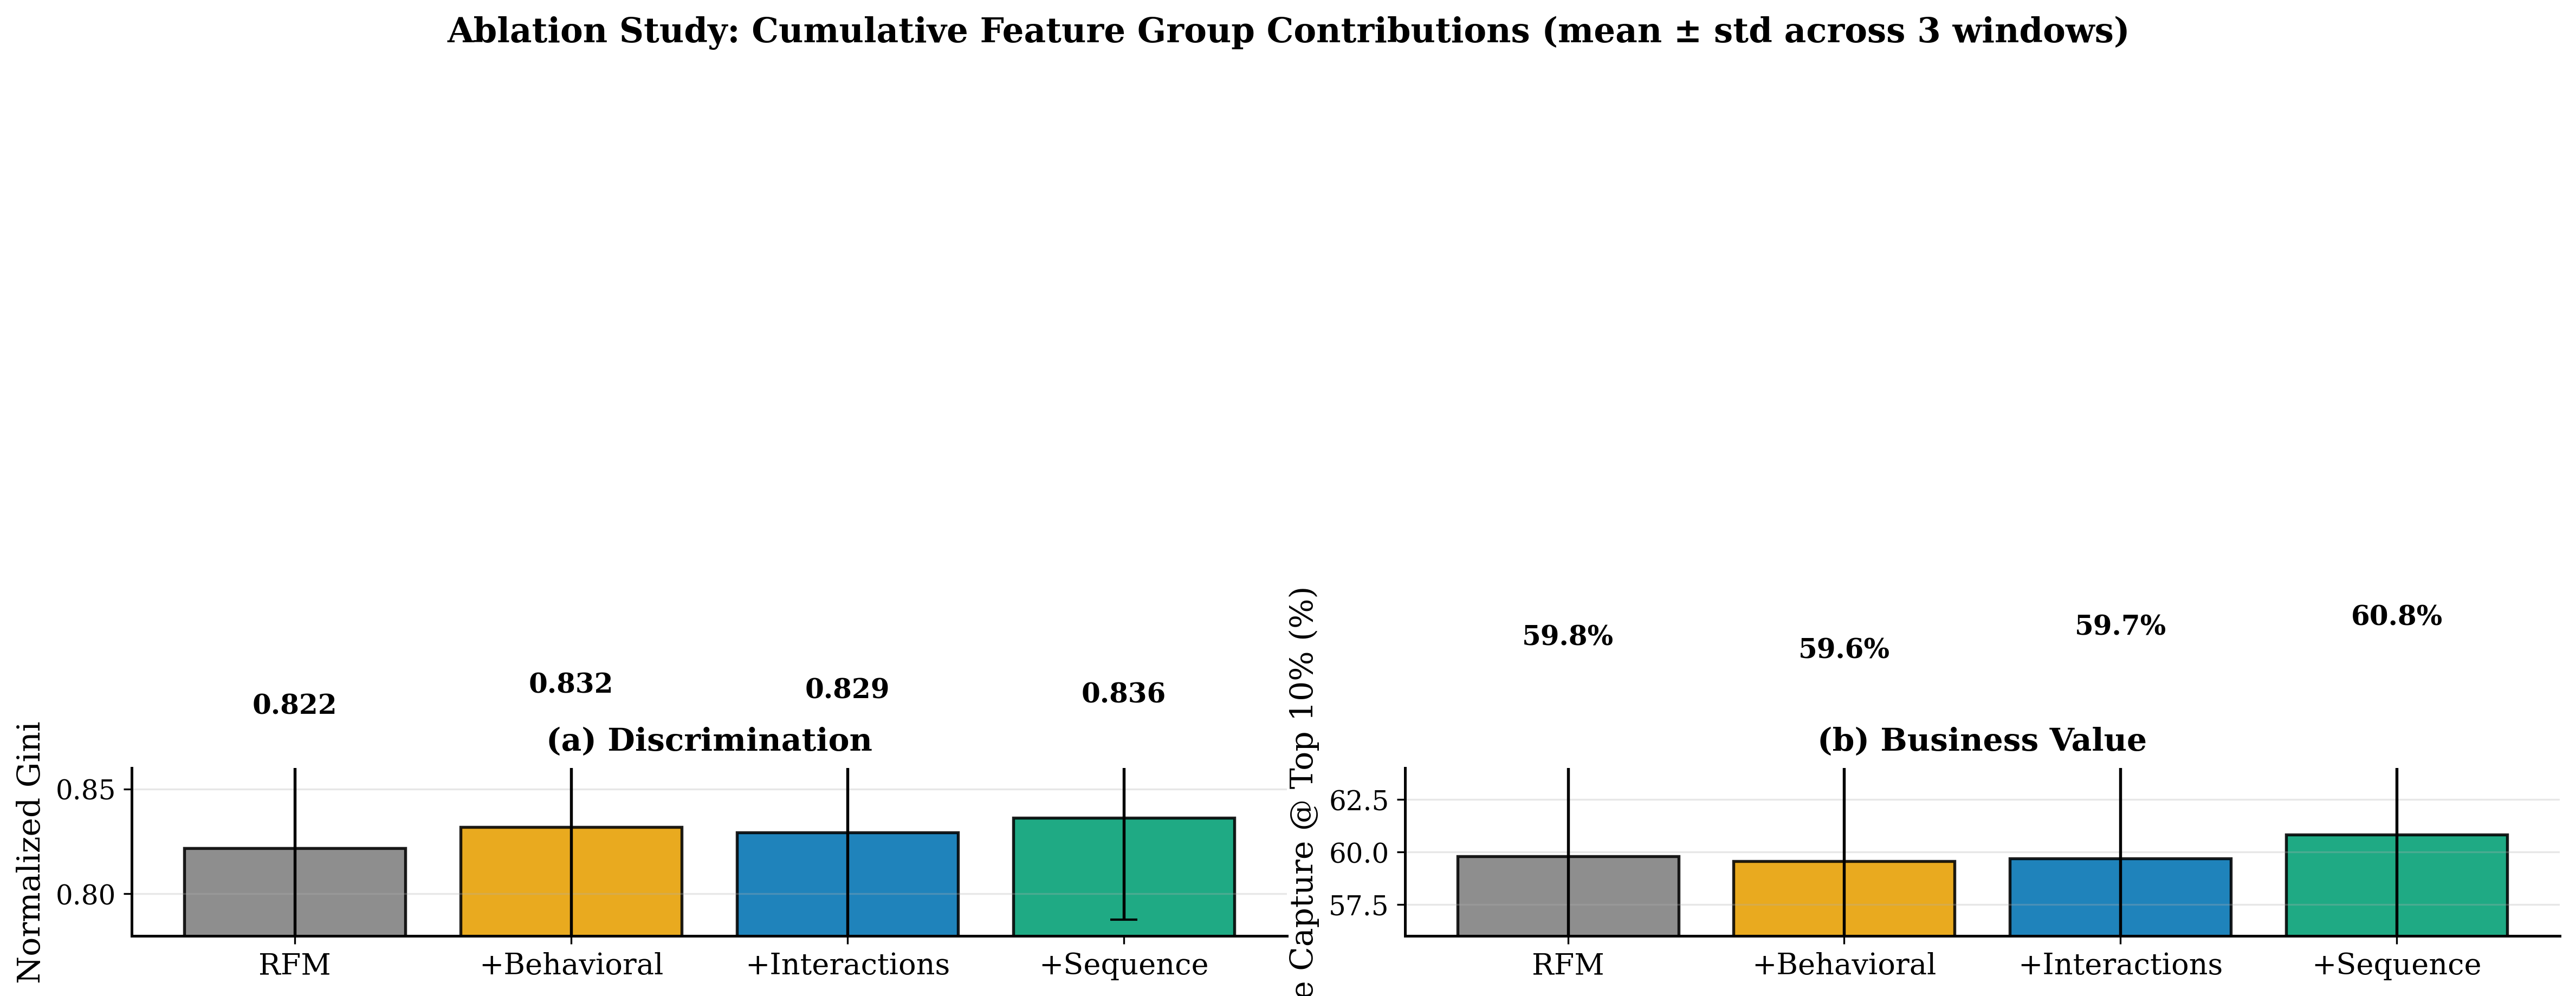
\includegraphics[width=0.9\textwidth]{../results/figures/fig5_ablation.png}
\caption{Feature group ablation study across all three walk-forward windows
(Hurdle Model with Optuna-tuned LightGBM). Error bars show window-to-window
variation. Adding monthly sequence features yields the single largest mean
improvement of $+0.015$ Normalized Gini over the RFM-only baseline.}
\label{fig:ablation}
\end{figure}

Fig.~\ref{fig:ablation} reports the ablation across three windows.
Starting from RFM-only (NG 0.822), behavioural features add $+0.010$,
interactions add $+0.008$, and monthly-sequence features add the
largest single gain ($+0.015$, NG 0.836). Although sequence features
provide a modest standalone NG uplift, they account for $\sim 24\%$
of total feature importance (Sec.~\ref{sec:shap}).

\textit{Stage-wise diagnostics.} On the stratified 80/20 test fold
across W1--W3, the Stage-1 classifier averages AUC-ROC
$0.798 \pm 0.018$ and AUC-PR $0.759 \pm 0.074$ (all metrics on the
held-out test set, fixed LightGBM hyperparameters). Semantic-variant
S1-AUC values in Table~\ref{tab:sem_variants} use Optuna-tuned
LightGBM over five windows and therefore differ slightly
($0.787$--$0.791$ vs.\ $0.798$); both are test-fold scores, not
validation-fold estimates. The Stage-2 regressor achieves
$R^2 = 0.407 \pm 0.106$ and MAE \$776~$\pm 334$ on the positive
subset. On Window~3, the Hurdle top-decile captures 65.07\% of actual
revenue versus 0.12\% in the bottom decile ($524\times$
discrimination).

\subsection{Explainability and Walk-Forward Stability}%
\label{sec:shap}

\begin{figure}[h]
\centering
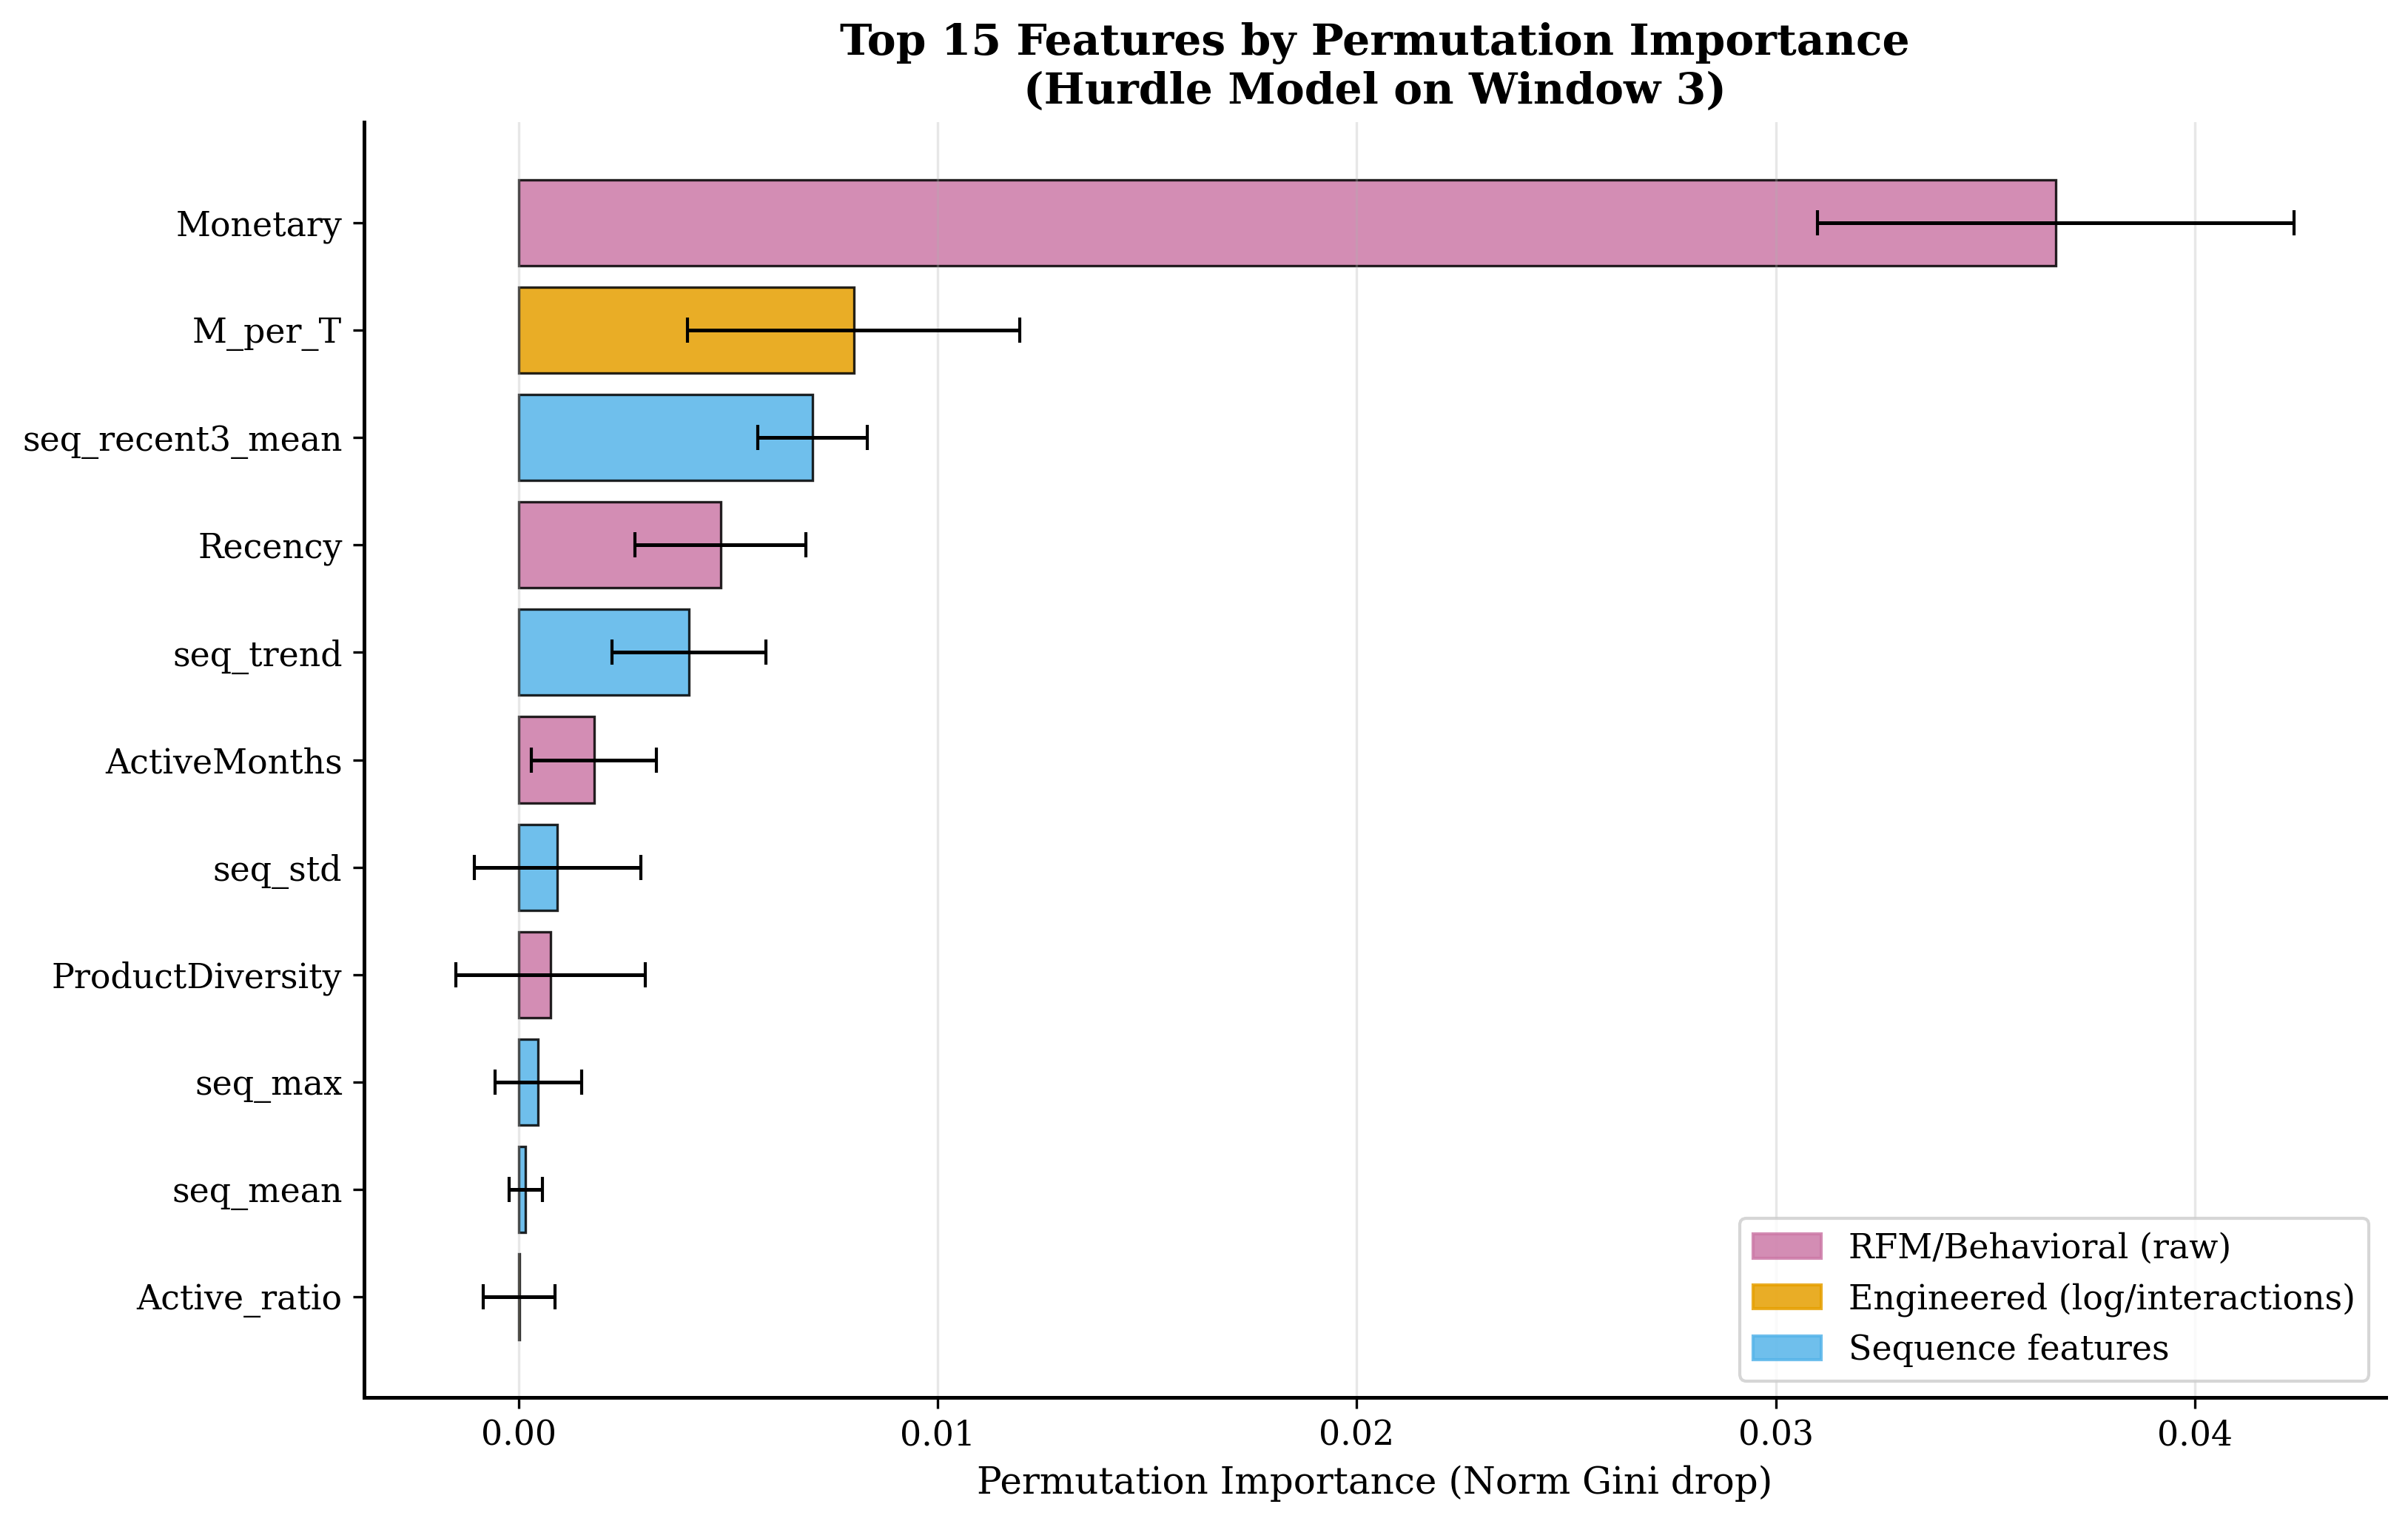
\includegraphics[width=\columnwidth]{../results/figures/fig7_importance.png}
\caption{Top 15 features by permutation importance for the Hurdle Model
on Window~3. Monetary leads (0.037), followed by M/T and
\texttt{seq\_recent3\_mean}; sequence features cumulatively account for
$\sim$24\% of total importance.}
\label{fig:importance}
\end{figure}

Monetary leads permutation importance (0.037), followed by M/T and
\texttt{seq\_recent3\_mean}. SHAP: Stage~1 is driven by ActiveMonths
($|\mathrm{SHAP}|{=}0.291$), Recency (0.255), and
\texttt{seq\_recent3\_mean} (0.197); Stage~2 by Monetary (0.365) and M/T
(0.155). All advanced models maintain NG $>0.77$ across five windows.

\subsection{Semantic Product Graph Feature Analysis}
\label{sec:sem_results}

Two refinements support semantic analysis: \textbf{supervised dimension
selection} (top-$K{=}8$ dims by training-fold Spearman correlation) and
\textbf{recency-aware profiling} (full-period and 90-day profiles plus
drift; Sec.~\ref{sec:semantic}).

\begin{table}[h]
\caption{Hurdle Model Variants Across Five Walk-Forward Windows
(mean $\pm$ std, $n{=}5$). \textsc{SemV2} = supervised top-8 +
recency-aware features (19 features). Bold marks the best per column.
S1-AUC is Stage-1 AUC-ROC on the stratified 80/20 \emph{test} fold with
Optuna-tuned LightGBM (15 trials); fixed-hyperparameter diagnostics on
W1--W3 yield mean $0.798 \pm 0.018$ (Sec.~\ref{sec:results}).}
\label{tab:sem_variants}
\small
\begin{tabular*}{\columnwidth}{@{\extracolsep\fill}lrrrr@{}}
\toprule
\textbf{Variant} & \textbf{N} & \textbf{NG} & \textbf{RC@10\%} &
\textbf{S1-AUC (test)} \\
\midrule
Hurdle-RFM    & 16 & $\mathbf{0.794{\pm}.067}$ & $56.82{\pm}8.9$ & $0.787$ \\
Hurdle-Seq    & 23 & $0.788{\pm}.079$ & $56.70{\pm}9.1$ & $0.789$ \\
Hurdle-SemV2  & 35 & $0.791{\pm}.074$ & $\mathbf{57.00{\pm}9.0}$ & $\mathbf{0.791}$ \\
Hurdle-AllV2  & 43 & $0.782{\pm}.083$ & $56.70{\pm}8.9$ & $0.782$ \\
\bottomrule
\end{tabular*}
\end{table}

\textsc{Hurdle-SemV2} achieves the highest mean RC@10\% (57.00\%).
Paired $t$-tests against \textsc{Hurdle-RFM} yield $p \geq 0.35$ for
NG, RC@10\% and test-fold Stage-1 AUC---semantic features do not
produce statistically significant aggregate ranking gains at $n{=}5$.

\textit{Interpretability.} SHAP on \textsc{Hurdle-AllV2} (W3) shows
semantic features account for 24.5\% of Stage-2 importance; six
$K$-means taste clusters are near-orthogonal to RFM (ARI 0.032) with
mean CLV \$484--\$1{,}531 ($p{=}4.5\!\times\!10^{-5}$).

\subsection{Calibrated Prediction Intervals}
\label{sec:cqr_results}

MCD-ZILN's nominal 95\% MC-Dropout intervals cover only
$34.2\%\pm 9.6\%$ of test CLV values under heavy tails. Applying the
same split-conformal widening used by CQR raises MCD coverage to
$94.7\%\pm 0.8\%$, showing that \emph{calibration}, not model family,
is the primary bottleneck. We therefore apply Conformalized Quantile
Regression (CQR)~\cite{romano2019conformalized} to the Hurdle Model
($\alpha{=}0.05$) for deployable intervals with provable marginal
coverage.

\begin{figure}[h]
\centering
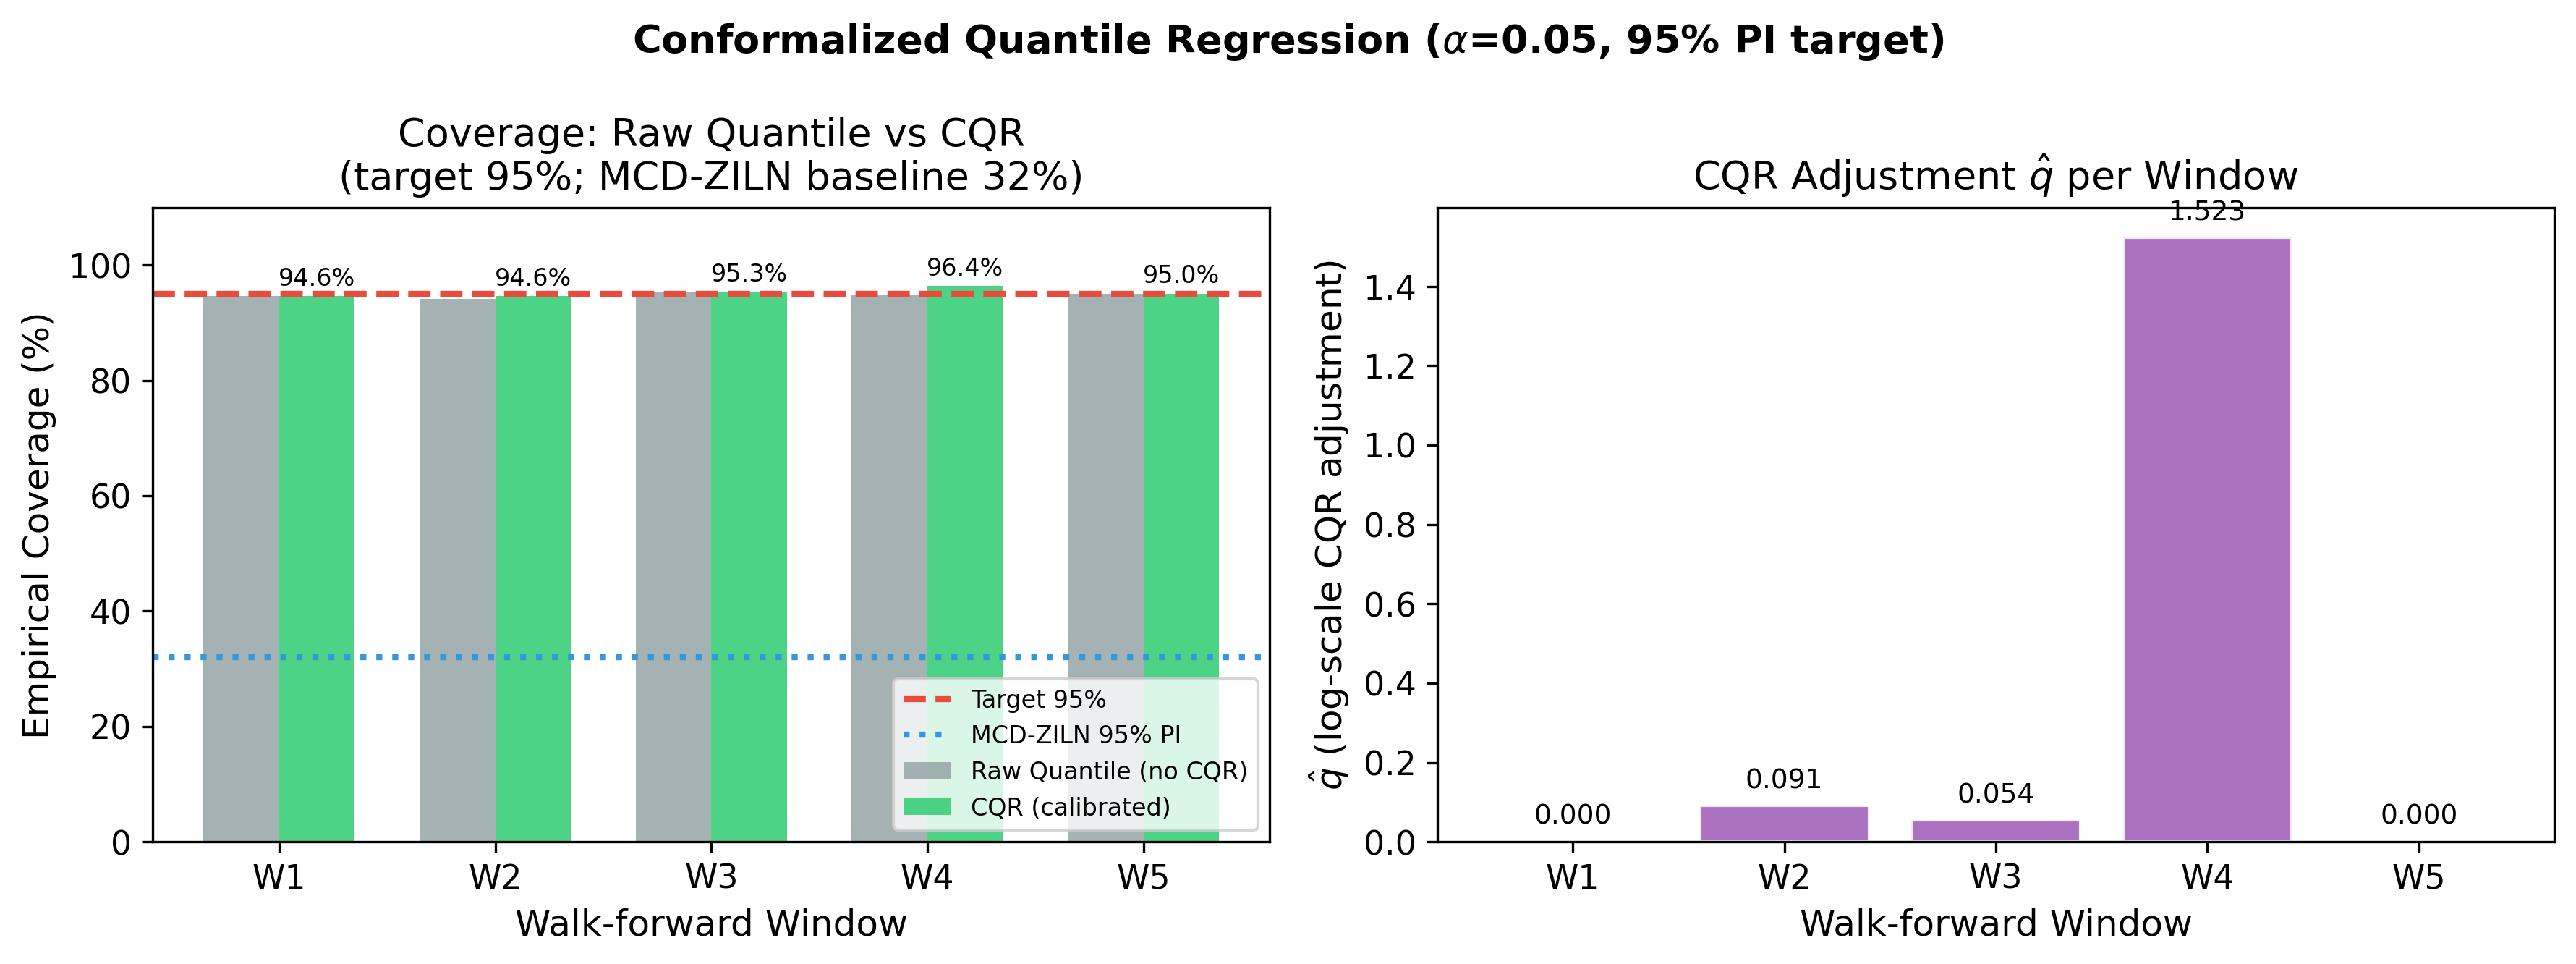
\includegraphics[width=\columnwidth]{../results/figures/fig_cqr_alpha05.png}
\caption{Conformalized Quantile Regression (CQR) coverage at
$\alpha{=}0.05$ (95\% target) across five walk-forward windows. Left:
raw-quantile vs.\ conformal-adjusted coverage, with the 95\% target.
Raw MCD MC-Dropout coverage (34.2\%) and split-conformal MCD (94.7\%) are
shown for reference (Table~\ref{tab:cqr}).}
\label{fig:cqr}
\end{figure}

\begin{table}[h]
\caption{CQR vs.\ conformal-calibrated MCD at $\alpha{=}0.05$ (95\% target).
All coverages are test-fold empirical values.}
\label{tab:cqr}
\small
\begin{tabular*}{\columnwidth}{@{\extracolsep\fill}lrrr@{}}
\toprule
\textbf{Method} & \textbf{Raw (\%)} & \textbf{Conf.\ (\%)} &
\textbf{Width (\$)} \\
\midrule
MCD-ZILN (MC Dropout) & 34.2 & 94.7 & 5{,}729 \\
CQR-Hurdle (quantile) & 94.8 & \textbf{95.2} & 1{,}607 \\
\bottomrule
\end{tabular*}
\end{table}

CQR-Hurdle achieves $\mathbf{95.2\%\pm 0.7\%}$ coverage with mean width
\$1{,}607---3.6$\times$ narrower than conformal-calibrated MCD
(\$5{,}729) at comparable coverage. Raw quantile coverage alone reaches
94.8\%; positive conformal correction $\hat q{>}0$ in three of five
windows. Midpoint ranking under CQR yields NG $0.792\pm0.057$ and
RC@10\% $55.29\%\pm 10.1$.

%% ============================================================
\section{Discussion}\label{sec:discussion}
%% ============================================================

\textit{Convergence and method selection.} Six top methods cluster at
NG 0.827--0.834 ($p\geq 0.12$). Method choice should follow secondary
criteria: interpretability favours Hurdle; deployable uncertainty favours
CQR-Hurdle; sequence-rich regimes favour dRNN/OptDist. Tree boosters match
deep models at this scale~\cite{grinsztajn2022treesvsnn}.

\textit{Hyperparameter tuning asymmetry.} Gradient-boosting models
received Optuna search (20 trials, 3-fold CV); deep baselines used
fixed Adam settings (Table~\ref{tab:deep_hparams}). We retain this
\emph{deliberate asymmetry} because deep training is 10--30$\times$
slower at $N{\approx}5{,}000$ and our focus is an interpretable
tree-first benchmark, not deep SOTA. We treat this deliberate
asymmetry as a feature of the study rather than a limitation, as it
reflects realistic scenarios where tree-based models are more
practical to tune on retail-scale data. We do \emph{not} interpret
comparable NG/RC@10\% as architectural inferiority. A pilot 10-trial
Optuna on ZILN (W3) yields test NG $0.884$ vs.\ $0.885$ fixed---negligible
and insufficient to break the NG${\approx}0.83$ ceiling.

\textit{dRNN dollar-scale calibration.} Table~\ref{tab:drnn_windows}
shows dRNN mean MAE (\$6{,}075) is driven by W1 (\$16{,}772;
$R^2{=}{-}155$); W2--W3 MAE is \$299--\$1{,}154 with NG
0.765--0.879. For VIP targeting we prioritise NG and RC@10\% over
aggregate MAE for sequence models.

\textit{Monetary baseline.} Historical-spend ranking achieves NG 0.822
and RC@10\% 60.02\%---only $-0.012$ NG behind the best learned method.
The Hurdle Model adds consistent MAE gains, two-stage SHAP, and semantic
taste clusters the Monetary baseline cannot produce.

\textit{Limitations.} (i)~The study uses a single UK retailer dataset
($N{=}5{,}038$). While this is a standard benchmark, results may not
fully generalize to other retail verticals or emerging markets;
cross-retailer validation is planned as future work.
(ii)~Five walk-forward folds limit statistical power.
(iii)~Deep baselines used fixed hyperparameters, while GBM models received
full Optuna tuning (deliberate asymmetry discussed in
Sec.~\ref{sec:discussion}).
(iv)~Stage-2 uses a homogeneous $\hat\sigma^2$ correction.
(v)~CQR and conformal MCD provide marginal, not conditional, coverage.
(vi)~Semantic predictive gains are not significant at $n{=}5$; value is
primarily interpretability and taste segmentation.

%% ============================================================
\section{Conclusion and Future Work}\label{sec:conclusion}
%% ============================================================

We presented a semantic knowledge-driven framework for CLV prediction
and VIP targeting on Online Retail~II. A two-stage Hurdle Model achieves
NG 0.834 and RC@10\% 60.96\% under walk-forward evaluation, comparable
to recent deep baselines while remaining interpretable. Semantic graph
features yield taste clusters orthogonal to RFM (ARI 0.03) and 24.5\%
Stage-2 SHAP importance, but not statistically significant aggregate
ranking gains ($p\geq 0.35$). CQR delivers 95.2\% coverage with
\$1{,}607 mean width; split-conformal calibration raises MCD-ZILN from
34.2\% to 94.7\% coverage, isolating calibration as the key uncertainty
issue. Future work will add deep hyperparameter parity across all windows,
heteroscedastic Stage-2 modelling, and cross-retailer validation.

%% ============================================================
%% DECLARATIONS (required by Springer Nature)
%% ============================================================

\bmhead{Acknowledgements} The author thanks the FPT University ADY201m
instructors and the UCI Machine Learning Repository.

\bmhead{Data and Code Availability} The Online Retail~II dataset is
publicly available at
\url{https://archive.ics.uci.edu/dataset/502/online+retail+ii}.
All implementation code and preprocessing scripts will be released
in a public repository upon acceptance, and are available from the
author on request in the meantime.

\bmhead{Conflict of Interest} The author declares none.

%% ============================================================
%% REFERENCES
%% ============================================================

\begingroup
\footnotesize
\setlength{\bibsep}{0pt plus 0.1ex}
\setlength{\itemsep}{0pt}
\setlength{\parskip}{0pt}
\setlength{\parsep}{0pt}
\begin{thebibliography}{30}

\bibitem{fader2005rfm}
Fader, P.S., Hardie, B.G.S., Lee, K.L.: RFM and CLV: Using iso-value curves
for customer base analysis. J. Market. Res. \textbf{42}(4), 415--430 (2005)

\bibitem{gupta2006clv}
Gupta, S., Hanssens, D., Hardie, B., Kahn, W., Kumar, V., Lin, N.,
Ravishanker, N., Sriram, S.: Modeling customer lifetime value.
J. Serv. Res. \textbf{9}(2), 139--155 (2006)

\bibitem{wang2019deep}
Wang, X., Liu, T., Miao, J.: A deep probabilistic model for customer lifetime
value prediction. arXiv preprint arXiv:1912.07753 (2019)

\bibitem{fader2005counting}
Fader, P.S., Hardie, B.G.S., Lee, K.L.: ``Counting your customers'' the easy
way: An alternative to the Pareto/NBD model. Market. Sci. \textbf{24}(2),
275--284 (2005)

\bibitem{fader2013gammagamma}
Fader, P.S., Hardie, B.G.S.: The Gamma-Gamma model of monetary value.
Technical note, University of Pennsylvania (2013)

\bibitem{tang2024optdist}
Tang, X., Li, Y., Wang, Y., Ruan, Y., Liu, Q., Chen, M., He, J.: OptDist:
Learning optimal distribution for customer lifetime value prediction. In:
Proc. 33rd ACM Int. Conf. Information and Knowledge Management (CIKM),
pp.~2200--2210 (2024)

\bibitem{meta2024drnn}
Chen, H., Ng, E., Smyl, S., Steininger, G.: Predicting customer lifetime value
using recurrent neural net. arXiv preprint arXiv:2412.20295 (2024).
Presented at the Customer Journey Optimization Workshop, KDD 2022

\bibitem{mcd2024clv}
Cao, X., Xu, Y., Yang, X.: Customer lifetime value prediction with uncertainty
estimation using Monte Carlo Dropout. arXiv preprint arXiv:2411.15944 (2024)

\bibitem{ke2017lightgbm}
Ke, G., Meng, Q., Finley, T., Wang, T., Chen, W., Ma, W., Ye, Q., Liu, T.Y.:
LightGBM: A highly efficient gradient boosting decision tree. In: Advances in
Neural Information Processing Systems, vol.~30, pp.~3146--3154 (2017)

\bibitem{akiba2019optuna}
Akiba, T., Sano, S., Yanase, T., Ohta, T., Koyama, M.: Optuna: A
next-generation hyperparameter optimization framework. In: Proc. 25th ACM
SIGKDD Int. Conf. Knowledge Discovery and Data Mining, pp.~2623--2631 (2019)

\bibitem{mullahy1986specification}
Mullahy, J.: Specification and testing of some modified count data models.
J. Econom. \textbf{33}(3), 341--365 (1986)

\bibitem{cragg1971statistical}
Cragg, J.G.: Some statistical models for limited dependent variables with
application to the demand for durable goods. Econometrica \textbf{39}(5),
829--844 (1971)

\bibitem{lundberg2017unified}
Lundberg, S.M., Lee, S.I.: A unified approach to interpreting model predictions.
In: Advances in Neural Information Processing Systems, vol.~30,
pp.~4765--4774 (2017)

\bibitem{chen2019online}
Chen, D.: Online Retail~II. UCI Machine Learning Repository (2019).
\url{https://archive.ics.uci.edu/dataset/502/online+retail+ii}

\bibitem{grinsztajn2022treesvsnn}
Grinsztajn, L., Oyallon, E., Varoquaux, G.: Why do tree-based models still
outperform deep learning on typical tabular data? In: Advances in Neural
Information Processing Systems, vol.~35, pp.~507--520 (2022)

\bibitem{romano2019conformalized}
Romano, Y., Patterson, E., Cand\`{e}s, E.: Conformalized quantile regression.
In: Advances in Neural Information Processing Systems, vol.~32,
pp.~3543--3553 (2019)

\bibitem{bullinaria2007extracting}
Bullinaria, J.A., Levy, J.P.: Extracting semantic representations from word
co-occurrence statistics: A computational study.
Behav. Res. Methods \textbf{39}(3), 510--526 (2007)

\bibitem{levy2014neural}
Levy, O., Goldberg, Y.: Neural word embedding as implicit matrix factorization.
In: Advances in Neural Information Processing Systems, vol.~27,
pp.~2177--2185 (2014)

\bibitem{linden2003amazon}
Linden, G., Smith, B., York, J.: Amazon.com recommendations: Item-to-item
collaborative filtering. IEEE Internet Comput. \textbf{7}(1), 76--80 (2003)

\end{thebibliography}
\endgroup

\end{document}
